% !TEX encoding = UTF-8
% !TEX TS-program = pdflatex
% !TEX root = ../tesi.tex

%**************************************************************
\chapter{Metodologia di sviluppo}
\label{cap:metodologia-lavoro}
%**************************************************************

\intro{In questo capitolo viene descritta la metodologia di lavoro e i ruoli adottati dal team di sviluppo.}\\

%**************************************************************
\section{Scrum}
\href{https://www.scrum.org/about}{Scrum} è un framework agile per lo sviluppo, consegna e manutenzione di prodotti software e non.
Scrum è progettato per l'utilizzo in team di dimensione ridotta. 
Di seguito vengono descritti ruoli, fasi e artefatti del framework.

\subsection{Ruoli}

\subsubsection{Scrum master}
Lo Scrum Master aiuta il team di sviluppo ad apprendere e applicare Scrum per conseguire valore di business. Lo Scrum Master fa tutto ciò che è in suo potere per aiutare il Team, il Product Owner e l'organizzazione ad avere successo. Lo ScrumMaster non è il manager dei membri del Team, né è un project manager, team leader, o rappresentante del team.
Lo scopo dello Scrum Master è:
\begin{itemize}
    \item aiutare a rimuovere gli ostacoli durante lo sviluppo;
    \item evitare interferenze esterne;
    \item aiutare il Team ad adottare al meglio le pratiche di sviluppo agile;
    \item fare in modo che tutti applichino Scrum nel miglior modo possibile.
\end{itemize}

\subsubsection{Product Owner}
Il Product Owner ha la responsabilità di massimizzare il ritorno sugli investimenti (ROI), di identificare le caratteristiche del prodotto, traducendole in una lista di priorità, di decidere cosa dovrebbe andare in cima alla lista per il prossimo Sprint, e di riassegnare le priorità, aggiornandole con continuità. Il Product owner detiene la responsabilità di profitto del prodotto, se questo è commerciale. In Agile il Product owner rappresenta il cliente e nell'applicazione di Scrum può e deve:
\begin{itemize}
    \item definire il Product Backlog, le user stories e gli acceptance criteria;
    \item definire le priorità nel Product Backlog e la data di rilascio del prodotto;
    \item accettare o rifiutare quanto sviluppato;
    \item cancellare lo sprint se risulta fallimentare o poco utile.
\end{itemize}


\subsubsection{Team di sviluppo}
Il team di sviluppo è composto da un insieme di persone, in genere meno di 10, e si occupa di sviluppare quanto definito dal product owner. Il team Scrum deve essere "cross-funzionale", ovvero includere tutte le competenze necessarie allo sviluppo del prodotto. I membri del team devono essere proattivi e aperti allo studio di tecnologie che vanno oltre le loro competenze.
Il team di sviluppo:
\begin{itemize}
    \item costruisce il prodotto definito dal Product owner;
    \item possiede tutte le conoscenze per ottenere un prodotto potenzialmente rilasciabile alla fine di ogni sprint;
    \item è auto organizzato, con un alto grado di autonomia e responsabilità;
    \item decide quanti e quali elementi del Product backlog sviluppare;
    \item ha la responsabilità di sviluppo, test e rilascio del prodotto;
    \item non possiede un team leader, in quanto in Scrum nel team di sviluppo sono considerati tutti di pari livello.
\end{itemize}

Nel corso dello stage i ruoli erano così suddivisi:
\begin{itemize}
    \item Scrum master: Bledar Gogaj
    \item Team di sviluppo: Alessandro Discalzi, Tania Parolin
    \item Product owner: Marco Lionello
\end{itemize}

\subsection{Artefatti}

\subsubsection{Product backlog}
Il Product backlog è un elenco di funzionalità, centrate sul cliente e ordinato per priorità; esiste e si evolve per tutta la durata del prodotto. Il Product backlog definisce quindi tutto ciò che deve essere fatto ed include una moltitudine di voci, più nello specifico:
\begin{itemize}
    \item nuove funzionalità da implementare;
    \item obbiettivi di miglioramento;
    \item lavori di ricerca;
    \item difetti da risolvere, se in numero contenuto;
\end{itemize}
Un buon Product backlog è \textbf{DEEP}:
\begin{itemize}
    \item \textbf{dettagliato}, con maggior attenzione alle voci di priorità più alta;
    \item \textbf{stimato}: per ogni voce deve esserci una stima per il completamento, la stima viene definita dal team di sviluppo;
    \item \textbf{emergente}: il Product backlog viene aggiornato in base alla variabilità del progetto;
    \item \textbf{prioritizzato}: le voci sono ordinate per priorità, quelle con priorità più alta forniscono maggior valore al prodotto.
\end{itemize}
Nel corso del progetto di stage per gestire il Product Backlog è stato utilizzato \href{https://taiga.io/}{Taiga}, un tool per la gestione di progetti agile.
\begin{figure}[h]
    \begin{center}
    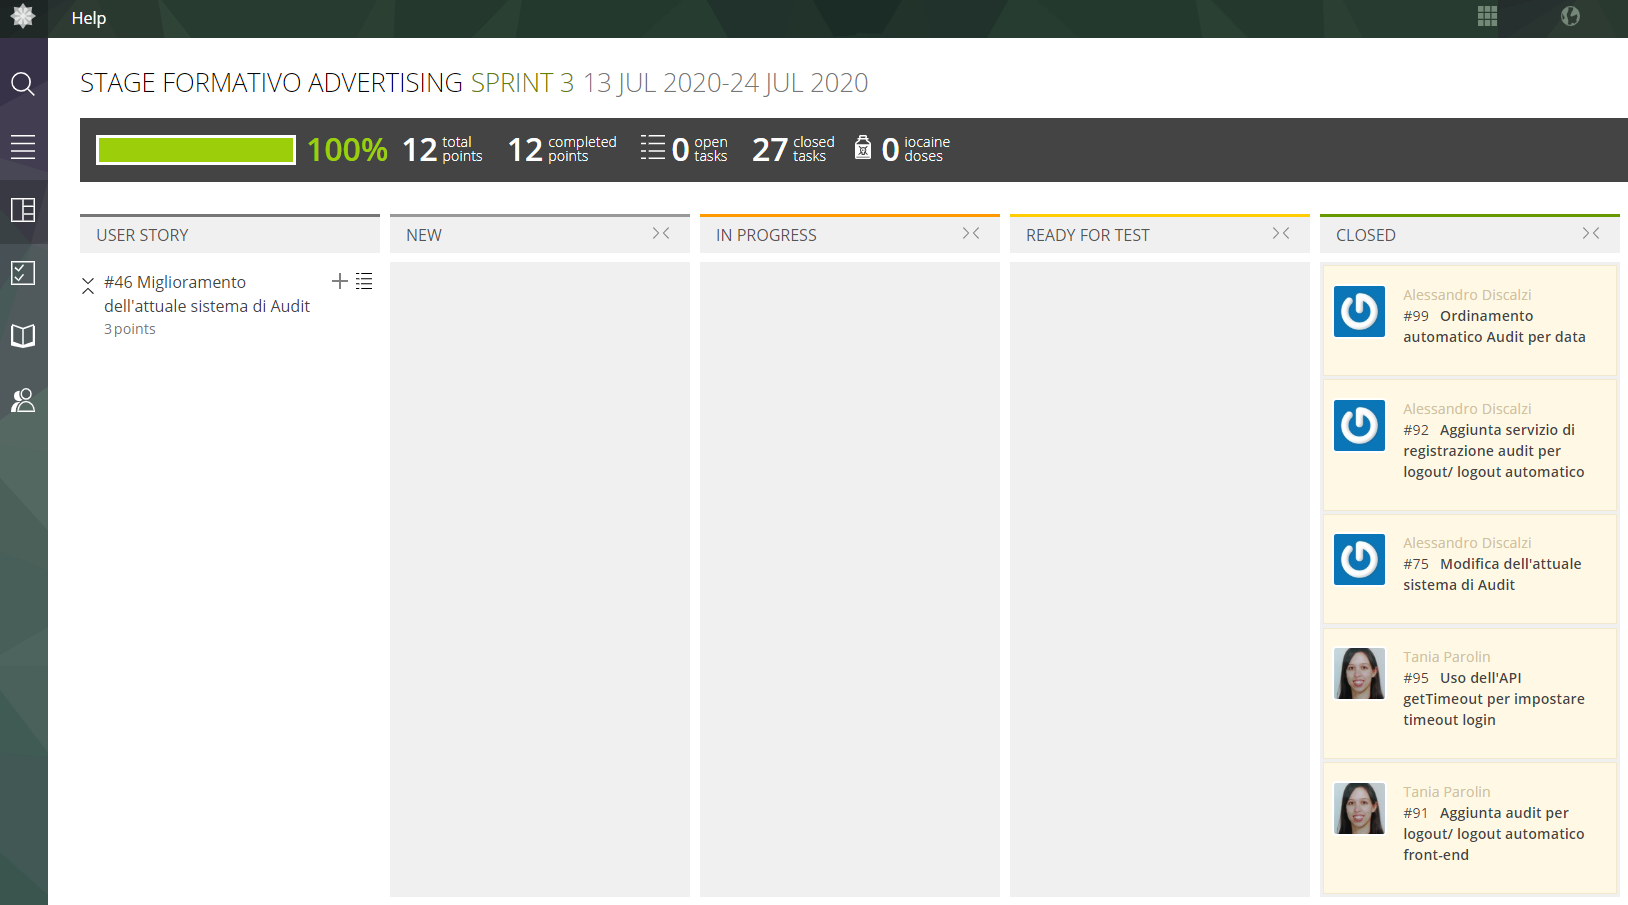
\includegraphics[width=1.2\textwidth]{taiga}
    \caption{Screenshot del backlog presente su Taiga rispetto uno degli sprint terminati}
    \label{fig:figure14}
    \end{center}
\end{figure}
\\Nel Product backlog di AMS la lista delle attività eseguite, in ordine di priorità, è la seguente:
\begin{itemize}
    \item design e realizzazione della base di dati;
    \item design e realizzazione del template di base per i contenuti pubblicitari;
    \item realizzazione della funzione di preview di un contenuto;   
    \item gestione autenticazione e autorizzazione in base ai ruoli;
    \item realizzazione dei servizi di back-end; 
    \item design e implementazione della \gls{ui}\glsfirstoccur{};
    \item integrazione front-end e back-end;
    \item implementazione della creazione di nuovi contenuti;
    \item implementazione della modifica di un contenuto;
    \item miglioramento \gls{ux}\glsfirstoccur{} e \gls{ui};
    \item inizio stesura documentazione;
    \item implementazione sistema di auditing;
    \item miglioramento dei contenuti di esempio;
    \item predisposizione di oracle;
    \item implementazione breadcrumbs;
    \item aggiunta controlli di validazione;
    \item completamento della documentazione;
    \item controlli sull'accessibilità del software;
    \item miglioramento pipeline di \gls{ci}\glsfirstoccur{};
    \item predisposizione demo.
\end{itemize}

\subsubsection{Definition of done}
Durante ogni sprint ciò che viene fatto costituisce un prodotto potenzialmente rilasciabile, questo deve essere approvato dal Product owner, dallo Scrum master e dal Team di sviluppo prima dell'inizio dello sprint successivo. La definition of done è un insieme di regole che definiscono quando ciò che viene fatto può essere definito rilasciabile.
La definition of done adottata durante lo stage è la seguente:
\begin{itemize}
    \item AMS (Advertising Management System) deve essere stato compilato senza warning;
    \item il software deve essere stato deployato nell’ambiente locale senza l'introduzione di nuovi errori e/o warning;
    \item devono essere stati eseguiti i test sulle nuove funzionalità;
    \item il codice deve essere stato revisionato dallo Scrum Master/Product Owner;
    \item la feature implementata deve essere accettata dal Product Owner.
\end{itemize}
Nei casi in cui questa definizione non fosse applicabile (ad esempio nel caso di modifiche che richiedono più voci/user stories/sprint) avrebbe dovuto essere evidenziata la violazione del Definition of Done allo Scrum Master ed al Product Owner ritardando la chiusura del Done a quando fosse stato effettivamente possibile.



\subsection{Fasi}

\subsubsection{Sprint}
Uno sprint è un periodo di tempo ben definito, di solito due settimane o un mese, durante il quale il team di sviluppo completa una parte di lavoro in base a quanto definito nel Product backlog.
Gli sprint hanno durata fissa che non può essere estesa, tuttavia se lo sprint risulta fallimentare o obsoleto può essere cancellato prima del termine dal Product owner.
\\Nel corso del progetto didattico la durata degli sprint è stata fissata a due settimane, mentre la durata e gli argomenti discussi durante le riunioni descritte successivamente hanno seguito le regole di Scrum.

\subsubsection{Sprint planning}
Lo sprint planning è un incontro che viene effettuato prima di ogni sprint, la cui durata è limitata a due ore per ogni settimana di sprint. L'obbiettivo dello sprint planning è definire cosa rilasciare al termine del prossimo sprint e come farlo.
Il lavoro da fare viene selezionato dal product backlog e inserito nello sprint anche in base alle stime di completamento definite dal team di sviluppo.

\subsubsection{Daily scrum}
Il Daily Scrum è una delle pratiche chiave di Scrum. Si tratta di un meeting giornaliero, della durata massima di 15 minuti, a cui partecipa il team di sviluppo, lo Scrum master e ,se richiesto, il Product owner. Il Daily scrum serve a sincronizzare il team e durante questo ogni membro deve rispondere a tre domande:
\begin{itemize}
    \item cosa è stato fatto dall'ultima riunione?
    \item cosa sarà fatto prima della prossima riunione?
    \item quali difficoltà si sono incontrate?
\end{itemize}
Nel caso alcuni ostacoli necessitino di discussioni approfondite queste possono essere fatte al termine del Daily scrum.

\subsubsection{Sprint review}
La sprint review si tiene alla fine di uno sprint, in modo da ispezzionare gli incrementi e aggiornare, se necessario, il Product backlog di conseguenza. Durante la sprint review il team di lavoro e gli stakeholders collaborano per vedere, in base a quanto fatto durante lo sprint, quali sono le prossime cose che si potrebbero fare per aumentare il valore del prodotto. La sprint review dura massimo un'ora per ogni settimana di sprint, durante la riunione si svolgono le seguenti attività:
\begin{itemize}
    \item il Product owner spiega quali attività del backlog sono state fatte e quali no;
    \item il team di sviluppo discute di cosa è andato bene, di cosa è andato storto e di come si sono affrontati i problemi durante lo sprint;
    \item il Team di sviluppo mostra il lavoro fatto e risponde ad eventuali domande riguardo l'incremento;
    \item se necessario il Product owner decide le date di rilascio in base a quanto fatto;
    \item il gruppo di lavoro collabora per decidere cosa fare prossimamente, questo serve anche come input allo sprint planning;
    \item review del potenziale di mercato del prodotto, se il prodotto è commerciale.
\end{itemize}

\subsubsection{Sprint retrospective}
La sprint retrospective ha luogo dopo la Sprint review e prima dello Sprint planning e la sua durata è limitata a 45 minuti per ogni settimana di sprint. Durante la retrospettiva, che viene vista come una possibilità di miglioramento per il team, si discute di cosa è andato bene, di cosa è andato storto e di come si può migliorare per il prossimo sprint. Questo favorisce il team in quanto si possono migliorare le metodologie adottate nello sprint precedente in base a ciò che è andato storto.